%2025 - 7a
\chapter{Dérivée covariante, connexion}
\section{07a Chapitre 5 : Dérivée covariante, connexion}

Motivation : dérivation de champs de vecteurs, de covecteurs ou de tenseurs dans une direction donnée

(M, $\mc{O}$, $\mc{A}$)


\begin{minipage}[c]{.5\linewidth}
\[
\begin{array}{ l c l l }
 \gamma : & \mb{R} & \to & M \\ 
  & \lambda & \mapsto & \gamma(\lambda) \\
\end{array}
\]
\begin{center}
Champ de vecteur $\mr{V}$

dérivée de $\mr{V}$

dans la direction X
\end{center}
\end{minipage}
\hfill
\begin{minipage}[c]{.5\linewidth}
\[
\begin{array}{ l l c l l }
 \gamma : &  {v}_{\gamma,p} : & \mc{C}^\infty(M) & \to & \mb{R} \\ 
  &  & f & \mapsto & {v}_{\gamma,p}(f)=(f\circ\gamma)'|_{\lambda_0} \\
X(f)  &  & df(X) & = & X(f) \\
\end{array}
\]
X(f) étant la dérivée de f dans la direction X
\[
\begin{array}{ l c l l }
 f : & M & \to & \mb{R} \\ 
  & p & \mapsto & f(p) \\
\end{array}
\]
\end{minipage}
\vspace{.3cm}

\begin{minipage}[c]{.45\linewidth}
$\mr{V}(q)-\mr{V}(p)$
\end{minipage}
\hfill
\begin{minipage}[c]{.45\linewidth}
$f(q)-f(p)$
\end{minipage}

\begin{minipage}[c]{.45\linewidth}
\[
\sigma M \to T M
\]
\[
\gamma (T M) 
\]
\end{minipage}
\hfill
\begin{minipage}[c]{.45\linewidth}
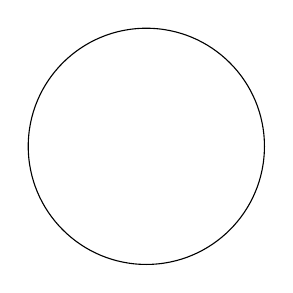
\begin{tikzpicture} % "THE GLOBE" showcase
\def\R{1.5} \def\angEl{35} % sphere radius, elevation angle
\draw (0,0) circle (\R);%\filldraw[ball] (0,0) circle (\R);
\foreach \t in {-80,-50,...,80} { \DrawLatitudeCircle[\R]{\t} }
\foreach \t in {10,-35,...,-150} { \DrawLongitudeCircle[\R]{\t} }
\end{tikzpicture}
\end{minipage}

\subsubsection{Contraintes à respecter : linéarité, règle(s) de Leibniz}

\begin{minipage}[c]{.45\linewidth}
\[
\nabla_V
\]
Vecteur autour d'un point

Champ de vecteur
\[
\nabla_\mr{V}
\]
\end{minipage}
\hfill
\begin{minipage}[c]{.45\linewidth}
\[
\nabla_V(f)\equiv V(f) = V^i \frac{\partial f}{\partial x^i}
\]
$\mr{V}_\gamma(f)=(f\circ\gamma)'$
\[
\nabla_V(f+g) = \nabla_V(f) + \nabla_V(g)
\]
\[
\nabla_{\alpha V}(f) = \alpha \nabla_V(f)
\]
\[
\nabla_{\rho V}(f) = \rho \nabla_V(f)
\]
\end{minipage}

\begin{minipage}[c]{.45\linewidth}
\[
\nabla_\mr{V}(T_1+T_2) = \nabla_\mr{V} (T_1) + \nabla_\mr{V} (T_2)
\]
\[
\nabla_{\mr{V}_1 + f \mr{V}_2}(T) = \nabla_{\mr{V}_1}(T) + f \nabla_{ \mr{V}_2}(T)
\]
\end{minipage}
\hfill
\begin{minipage}[c]{.45\linewidth}
\[
(fg)'=f'g+fg'
\]
\[
\lim_{dx \to 0} \frac{f(x+dx)g(x+dx) - f(x)g(x)}{dx}
\]
\end{minipage}


\begin{minipage}[c]{.45\linewidth}
\[
\nabla_\mr{V}(fT) = (\nabla_\mr{V} f)T + f (\nabla_\mr{V} T)
\]
\[
\nabla_\mr{V}(T_1\otimes T_2) = (\nabla_\mr{V} T_1)\otimes T_2 + T_1 \otimes \nabla_\mr{V} (T_2)
\]
T de rang $(1,1)$
\[
\nabla_V(T(\omega,X)) = (\nabla_V T)(\omega,X) + T(\nabla_V \omega,X) + T(\omega,\nabla_V X)
\]
\end{minipage}
\hfill
\begin{minipage}[c]{.45\linewidth}
\end{minipage}

\vspace{1cm}
$(\mc{U}, x)$ \hspace{1cm} $p\in\mc{U}$

\begin{minipage}[c]{.45\linewidth}
\[
\nabla_V W = \nabla_{V^i(\frac{\partial}{\partial x^i})}(W^j(\frac{\partial}{\partial x^i}) = V^i\nabla_{(\frac{\partial}{\partial x^i})}(W^j(\frac{\partial}{\partial x^j})
\]
\[
\nabla_V W = V^i(\nabla_{\frac{\partial}{\partial x^i}}W^j)(\frac{\partial}{\partial x^j})) + V^iW^j\nabla_{(\frac{\partial}{\partial x^i})}(\frac{\partial}{\partial x^j})
\]
\[
\qquad = V^i(\frac{\partial W^j}{\partial x^i})(\frac{\partial}{\partial x^j}) + V^iW^j
\]
\end{minipage}
\hfill
\begin{minipage}[c]{.45\linewidth}

\[
V = V^i(\frac{\partial}{\partial x^i})_p
\]
\[
W = V^j(\frac{\partial}{\partial x^j})_p
\]
\[
\nabla_{(\frac{\partial}{\partial x^i})}(\frac{\partial}{\partial x^j})
-> \mv{\Gamma}_{ji} = \Gamma^k_{\omega ji}(\frac{\partial}{\partial x^k})
\]
\end{minipage}


Choix libre de $(dim\ M)^2$ fonctions $\mc{C}^\infty$
\[
\Gamma^k_{\omega ji}(\frac{\partial}{\partial x^k}) \qquad composante
\]

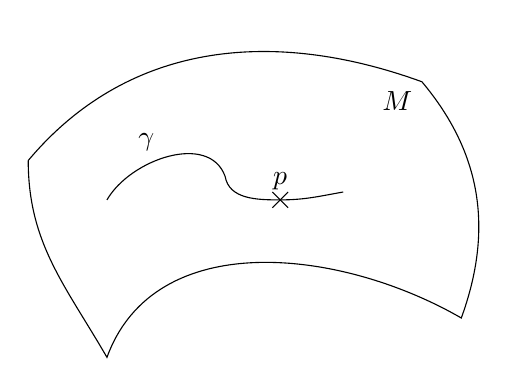
\begin{tikzpicture}
\draw(-3, 1) to[out=50, in=160] (2,2) node[below left]{$M$}
to[out=-50, in=70] (2.5,-1)
to[out=150, in=70] (-2,-1.5)
to[out=120, in=-90] (-3, 1); % Espace
%
\draw(-1.5,1) node[above]{$\gamma 	$};
\draw(-2,0.5) to[out=60, in=110] (-0.5,0.8)
to[out=-80, in=180]  (0.2,0.5) node[above]{$p$}
to[out=0, in=190] (1,0.6); % Courbe
%
\draw(0.1,0.6) -- (0.3,0.4);
\draw(0.1,0.4) -- (0.3,0.6);
\end{tikzpicture}

\begin{minipage}[c]{.45\linewidth}
{\large
\[
\Gamma^k_{\omega\ ji}
\]
}
\end{minipage}
\hfill
\begin{minipage}[c]{.45\linewidth}
composante de la dérivée du 
champ de vecteur $\frac{\partial}{\partial x^i}$
dans la direction $\frac{\partial}{\partial x^k}$
\end{minipage}

Coeficient de la connexion de la carte $(\mc{U}, x)$

{\large
\[
\Gamma^i_{\omega\ jk} = dx^i\left(\nabla_{\frac{\partial}{\partial x^k}}(\frac{\partial}{\partial x^j})\right)
\]
}
\vspace{1cm}


{\large
\[
\Gamma^a_{\omega\ bc} = dy^a\left(\nabla_{\frac{\partial}{\partial y^c}}
(\frac{\partial}{\partial y^b})\right)
=\frac{\partial y^a}{\partial x^i} dx^i \left
(\nabla_{\frac{\partial x^k}{\partial y^c} \frac{\partial}{\partial x^k}}
(\frac{\partial x^j}{\partial y^b} \frac{\partial}{\partial x^j})\right)
\]
\[
=\frac{\partial y^a}{\partial x^i} dx^i \left[
\frac{\partial x^k}{\partial y^c} \nabla_{ \frac{\partial}{\partial x^k}}
(\frac{\partial x^j}{\partial y^b} \frac{\partial}{\partial x^j})\right]
\]
\[
=\frac{\partial y^a}{\partial x^i} \frac{\partial x^k}{\partial y^c} dx^i
 \left[
 \nabla_{ \frac{\partial}{\partial x^k}} (\frac{\partial x^j}{\partial y^b}
 \frac{\partial}{\partial x^j}) + 
 \frac{\partial y^a}{\partial x^i} \nabla_{ \frac{\partial}{\partial x^k}}
 \frac{\partial}{\partial x^j} \right]
\]
}
\vspace{1cm}

\begin{minipage}[c]{.45\linewidth}
{\large
\[
\Gamma^a_{\omega\ bc} = dy^a\left(\nabla_{\frac{\partial}{\partial y^c}}
(\frac{\partial}{\partial y^b})\right)
=\frac{\partial y^a}{\partial x^i} dx^i \left
(\nabla_{\frac{\partial x^k}{\partial y^c} \frac{\partial}{\partial x^k}}
(\frac{\partial x^j}{\partial y^b} \frac{\partial}{\partial x^j})\right)
\]
}
\end{minipage}
\hfill
\begin{minipage}[c]{.45\linewidth}
\end{minipage}
Liberté restante : coefficient d'une connexion

Dérivée covariante de champs de tenseurs de rang quelconque

Transformation des coefficients de la connexion lors d'un changemment de carte
